\section{Dark enrgy models}
\begin{figure}
	\centering
	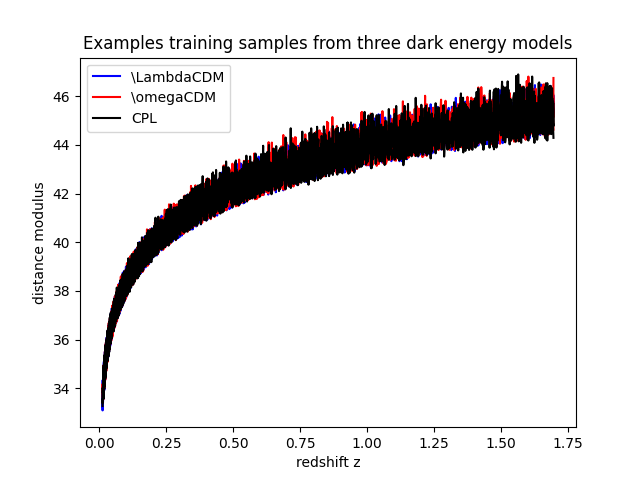
\includegraphics[width=\textwidth]{dark_energy/samples.png}
	\caption{Samples from dark energy models}
	\label{fig:dark_energy_samples}
\end{figure}
We consider three popular dark energy models to test out VAE-GAN network for model selection and interpolation.
\subsection{$\Lambda$CDM}
The equation of state parameter is
\begin{equation}
	\omega(z)=-1
\end{equation}
\subsection{$\omega$CDM}
\begin{equation}
	\omega(z)=\omega_{D E}
\end{equation}
\subsection{CPL}
\begin{equation}
	\omega(z)=\omega_{0}+\omega_{a} \frac{z}{1+z}
\end{equation}
\subsection{Distance Modulus}
We evaluate these models at redshifts $z_{obs}$ given by Union2.1 data and randomly sampled redshifts between $(0.8 min(z_{obs}) - 1.2 * max(z_{obs})$. The expansion rate of a spatially flat FRW universe is determined by the matter and dark energy,
$$
H^{2}(z)=H_{0}^{2}\left\{\Omega_{m 0}(1+z)^{3}+\left(1-\Omega_{m 0}\right) \exp \left[3 \int \frac{1+\omega\left(z^{\prime}\right)}{1+z^{\prime}} d z^{\prime}\right]\right\}
$$
The luminosity distance is closely related to the Hubble expansion rate (Eq.12), and the distance modulus is given by $\mathrm{Eq} 13$
$$
\begin{gathered}
D_{L}(z)=c(1+z) \int_{0}^{z} d z^{\prime} \frac{1}{H\left(z^{\prime}\right)} \\
\mu(z)=5 \log _{10} D_{L}(z)+25
\end{gathered}
$$
For each dark energy model, 12800 samples are generated at the redshift $\boldsymbol{z}=\operatorname{sort}\left\{\boldsymbol{z}_{\text {obs }}, \boldsymbol{z}^{*}\right\}$, given the priors of the parameters as,
$$
\begin{aligned}
\Omega_{m 0} & \sim \mathcal{U}(0.1,0.9) \\
H_{0} & \sim \mathcal{U}(50,90) \\
\omega_{D E} & \sim \mathcal{U}(-1.8,-0.4) \\
\omega_{0} & \sim \mathcal{U}(-1.9,-0.4) \\
\omega_{a} & \sim \mathcal{U}(-4.0,4.0)
\end{aligned}
$$
$\boldsymbol{z}^{*}$ has 1468 elements evenly located in the interval, $\left[0.8 \min \left(\boldsymbol{z}_{o b s}\right), 1.2 \max \left(\boldsymbol{z}_{o b s}\right)\right]$. The $12800 \times 3$ samples
\begin{figure}
	\centering
	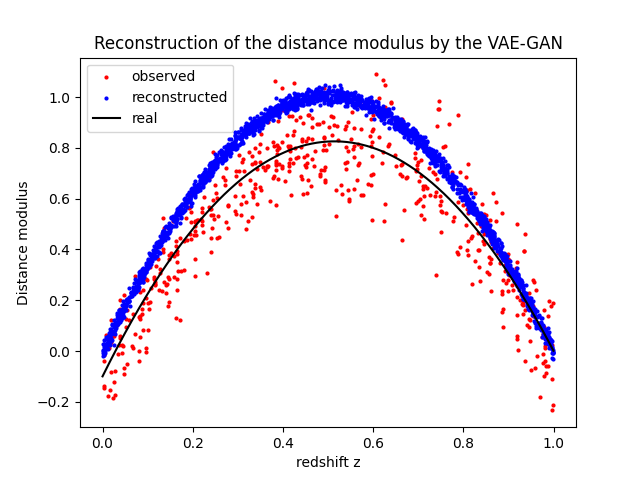
\includegraphics[width=\textwidth]{dark_energy/true_vs_reconstructed.png}
	\caption{Reconstruction}
	\label{fig:recon_de}
\end{figure}